\begin{frame}{Qu'est-ce qu'un profil?}
    \begin{itemize}
        \item Objet ambigü: toujours à moitié montré (donc à moitié caché)
        \item Une écriture de soi consciente et inconsciente.
        \item Les réseaux sociaux nous écrivent également pendant que nous écrivons.
    \end{itemize}
\end{frame}

\begin{frame}{Qu'est-ce qu'un profil?}
    \textbf{L'art de la silhouette}
    \vspace{3em}
    \begin{columns}
    % Colonne de gauche : Texte
        \begin{column}{0.4\textwidth}
            \begin{itemize}
                \item Mythe de Dibutade.
                \item Se superpose à l'émergence de l'individualité: la silhouette fait de nous quelqu'un d'unique.
            \end{itemize}
        \end{column}

        % Colonne de droite : Image
        \begin{column}{0.5\textwidth}
            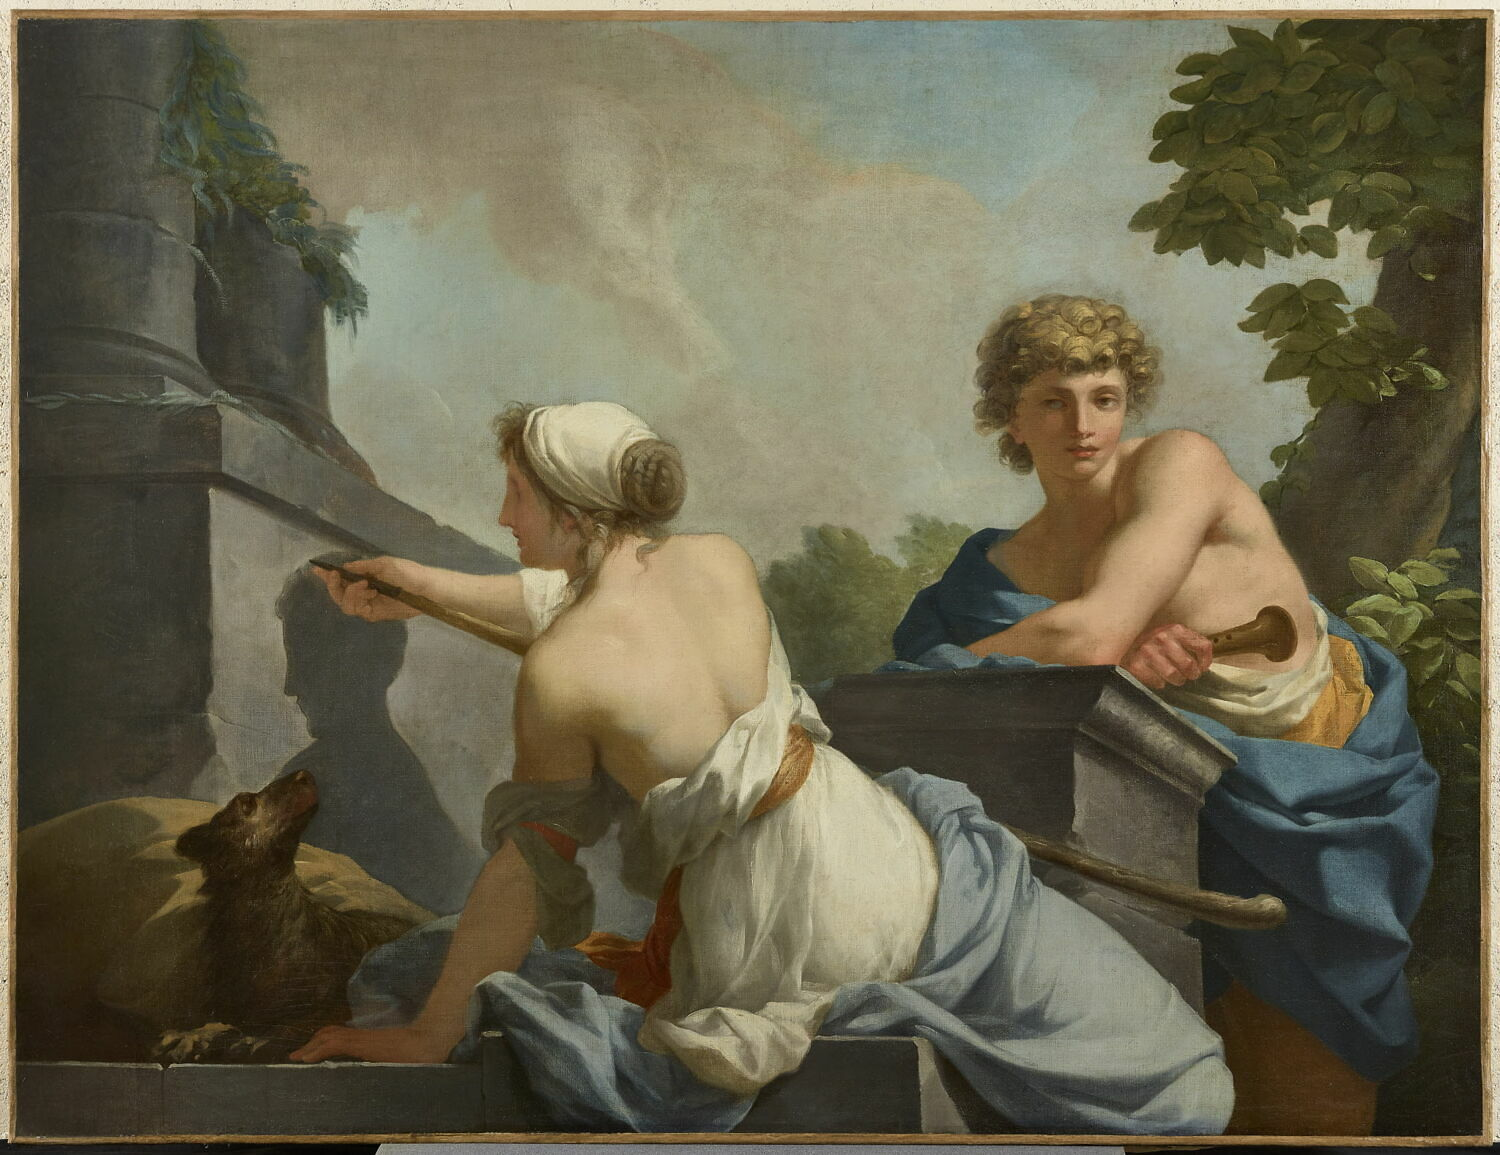
\includegraphics[width=.9\columnwidth]{Images/regnault_origine_peinture.JPG}
            
        \end{column}
    \end{columns}
    
\end{frame}

\begin{frame}{Qu'est-ce qu'un profil?}
    \begin{block}{Le profil: une notion de psychanalyse}
        \textrightarrow{} Vient désigner les principaux traits caractéristiques d'un individu.
    \end{block}
    \begin{block}{Le profil professionnel}
        \textrightarrow{} Compétences de chasseur de têtes.        
    \end{block}
    \begin{block}{Enfin, le profil numérique}
        \textrightarrow{} Une écriture consciente et maîtrisée
        \textrightarrow{} Une écriture latente
        
    \end{block}
\end{frame}

\begin{frame}{Les enjeux critiques}
\begin{enumerate}
    \item \textbf{Concurrence (sujet vs logiciel)}: autonomie ou hétéronomie? Dans quelle mesure notre identité numérique est déterminée et influencée par les outils ou les plateformes numériques?
    \item \textbf{Concordance (sujet // logiciel)}: réflexion sur les études algorithmiques. Algorithmes "prédictifs"?
    \item \textbf{Surveillance (sujet < logiciel)}: la machine n'est-elle là que pour mieux m'espionner ou me contrôler? 
\end{enumerate}

\end{frame}